%Группа 11-3 Модуль 2
\title{Занятие №1}
\begin{listofex}
	\item В школе есть трехместные туристические палатки. Какое наименьшее число палаток нужно взять в поход, в котором участвует 20 человек? \answer{ 7 }
	\item Больному прописано лекарство, которое нужно пить по 0,5 г 3 раза в день в течение 21 дня. В одной упаковке 10 таблеток лекарства по 0,5 г. Какого наименьшего количества упаковок хватит на весь курс лечения?\answer{ \( 7 \) }
	\item Для ремонта квартиры требуется 63 рулона обоев. Сколько пачек обойного клея нужно купить, если одна пачка клея рассчитана на 6 рулонов? \answer{ \( 11 \) }
	\item Стоимость проезда в маршрутном такси составляет 20 руб. Какое наибольшее число поездок можно будет совершить в этом маршрутном такси на 150 руб., если цена проезда снизится на 10\%? \answer{ 11 }
	\item Таксист за месяц проехал 6000 км. Стоимость 1 литра бензина — 20 рублей. Средний расход бензина на 100 км составляет 9 литров. Сколько рублей потратил таксист на бензин за этот месяц? \answer{ \( 10800 \) }
	\item 1 киловатт-час электроэнергии стоит 1 рубль 80 копеек. Счетчик электроэнергии 1 ноября показывал 12 625 киловатт-часов, а 1 декабря показывал 12802 киловатт-часа. Сколько рублей нужно заплатить за электроэнергию за ноябрь? \answer{ \( 381,6 \) }
	\item Установите соответствие между величинами и их возможными значениями: к каждому элементу первого столбца подберите соответствующий элемент из второго столбца.
	\begin{center}
		
\includegraphics[width=0.8\linewidth]{125.jpg}
	\end{center}
	В таблице под каждой буквой, соответствующей величине, укажите номер её возможного значения.
	\begin{center}
		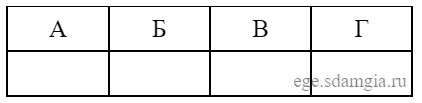
\includegraphics[width=0.4\linewidth]{126.jpg}
	\end{center}
	\item Решить уравнение:
	\begin{enumcols}[itemcolumns=1]
		\item \exercise{459}
		\item \exercise{493}
		\item \exercise{3669}
		\item \exercise{500}
		\item \exercise{509}
	\end{enumcols}
\end{listofex}
\newpage
\title{Домашняя работа №1}
\begin{listofex}
	\item В доме, в котором живет Петя, один подъезд. На каждом этаже находится по 6 квартир. Петя живет в квартире № 50. На каком этаже живет Петя? \answer{ 9 }
	\item Ананасы стоят 85 руб. за штуку. Какое максимальное число ананасов можно купить на 500 руб., если их цена снизится на 20\%? \answer{ 7 }
	\item Спидометр автомобиля показывает скорость в милях в час. Какую скорость (в милях в час) показывает спидометр, если автомобиль движется со скоростью 36 км в час? (Считайте, что 1 миля равна 1,6 км.) \answer{ \( 22,5 \) }
\end{listofex}
%\newpage
%\title{Занятие №2}
%\begin{listofex}
%
%\end{listofex}
%\newpage
%\title{Занятие №3}
%\begin{listofex}
%
%\end{listofex}
%\newpage
%\title{Занятие №4}
%\begin{listofex}
%
%\end{listofex}
%\newpage
%\title{Домашняя работа №2}
%\begin{listofex}
%
%\end{listofex}
%\newpage
%\title{Занятие №5}
%\begin{listofex}
%
%\end{listofex}
%\newpage
%\title{Занятие №6}
%\begin{listofex}
%
%\end{listofex}
%\newpage
%\title{Занятие №7}
%\begin{listofex}
%
%\end{listofex}
%\newpage
%\title{Проверочная работа}
%\begin{listofex}
%
%\end{listofex}